\section{Cơ sở lý thuyết}
\subsection{Tổng quan về dữ liệu chuỗi thời gian và luồng dữ liệu thời gian thực}
\subsubsection{Dữ liệu chuỗi thời gian đa biến}
    \subsubsection*{Khái niệm}
    
    Chuỗi thời gian là một chuỗi các quan sát được ghi nhận tuần tự theo thời gian. Khi quá trình quan sát theo dõi đồng thời nhiều biến số khác nhau từ cùng một hệ thống động, dữ liệu thu được gọi là chuỗi thời gian đa biến (Multivariate Time-Series).
    
    Về mặt toán học, một chuỗi thời gian đa biến $X$ có độ dài $T$ được định nghĩa là một tập hợp các vector:
    $$X = \{x_1, x_2, \dots, x_T\}$$
    Trong đó, tại mỗi bước thời gian $t \in \{1, 2, \dots, T\}$, quan sát $x_t$ là một vector thuộc không gian $d$ chiều ($x_t \in \mathbb{R}^d$), với $d$ là tổng số lượng các biến được quan sát. Mỗi phần tử $x_{t, i}$ ($i = 1, 2, \dots, d$) đại diện cho giá trị của biến số thứ $i$ tại thời điểm $t$. Toàn bộ chuỗi thời gian đa biến có thể được biểu diễn dưới dạng một ma trận $X \in \mathbb{R}^{T \times d}$.
    
    \subsubsection*{Đặc trưng cấu trúc}
    
    Khác với dữ liệu tĩnh truyền thống—nơi các mẫu quan sát thường được giả định là độc lập và phân phối đồng nhất — chuỗi thời gian đa biến bị chi phối bởi hai cấu trúc phụ thuộc thống kê cốt lõi:
    \begin{itemize}[label=--]
        \item \textbf{Phụ thuộc thời gian}: Trạng thái của vector quan sát tại thời điểm $t$ không độc lập mà có mối liên hệ trói buộc với các trạng thái trong quá khứ. Xét theo lý thuyết xác suất, phân phối có điều kiện của $x_t$ phụ thuộc vào chuỗi dữ liệu lịch sử trước đó: $P(x_t | x_{t-1}, x_{t-2}, \dots) \neq P(x_t)$. Tính chất tự tương quan này phản ánh quán tính, xu hướng và tính tuần hoàn của hệ thống động theo thời gian.
        \item \textbf{Phụ thuộc không gian / Tương quan chéo}: Tại một thời điểm $t$ bất kỳ, $d$ biến số thành phần bên trong vector $x_t$ không hoạt động độc lập một cách ngẫu nhiên. Ma trận hiệp phương sai sinh ra từ các biến số này thường không phải là ma trận đường chéo, thể hiện sự tương tác và đồng biến động giữa chúng. Trong phân tích đa biến, việc mô hình hóa không chỉ nhằm nắm bắt hành vi đơn lẻ của từng biến, mà trọng tâm là phải học được phân phối kết hợp  của không gian $d$ chiều. Một sự kiện bất thường có thể không biểu hiện qua một outlier trên một biến đơn lẻ, mà biểu hiện qua sự phá vỡ cấu trúc tương quan lịch sử đã được thiết lập giữa nhiều biến số.
    \end{itemize}
\subsubsection{Đặc điểm của luồng dữ liệu thời gian thực}
    \subsubsection*{Khái niệm}
    
    Dòng dữ liệu là một chuỗi các phần tử dữ liệu có thể đếm được, được sinh ra liên tục theo thời gian với tốc độ cao, trong đó số lượng phần tử có thể được xem là gần như vô hạn.\\% Ref
    Về mặt toán học, một dòng dữ liệu $S$ có thể được biểu diễn như một chuỗi các quan sát được sinh ra theo thời gian:
    $$S = \{x_1, x_2, \dots, x_t, \dots\}$$
    Trong đó, $x_t$ là phần tử dữ liệu (hoặc một véc-tơ đặc trưng) đến hệ thống tại thời điểm $t$. 
    
    \subsubsection*{Đặc trưng}
    
    Khác với khai phá dữ liệu truyền thống (thường áp dụng trên các cơ sở dữ liệu quan hệ), khai phá dòng dữ liệu mang những đặc trưng cốt lõi sau:
    \begin{itemize}[label=--]
        \item \textbf{Tính vô hạn và liên tục}: Dữ liệu đến liên tục và không có điểm kết thúc định trước. Do đó, không thể lưu trữ toàn bộ dòng dữ liệu vào bộ nhớ vật lý hoặc đĩa cứng để xử lý dần.
        \item \textbf{Truy cập một lần}: Thuật toán chỉ có thể nhìn thấy mỗi phần tử dữ liệu $x_t$ một lần duy nhất khi nó vừa đến. Sau khi xử lý, phần tử này sẽ bị loại bỏ hoặc tóm tắt lại, không thể truy xuất lại dữ liệu gốc một cách ngẫu nhiên.
        \item \textbf{Tốc độ cao}: Tốc độ sinh dữ liệu thường rất lớn, đòi hỏi hệ thống phải tính toán và đưa ra kết quả trong một khoảng thời gian cực kỳ nghiêm ngặt (thường tính bằng mili-giây).
    \end{itemize}
    Trong các hệ thống giám sát hiện đại, dữ liệu thường được sinh ra dưới dạng các dòng dữ liệu liên tục, chẳng hạn như các chỉ số hiệu năng hệ thống, dữ liệu cảm biến hoặc nhật ký hệ thống. Việc phân tích và phát hiện bất thường trên các dòng dữ liệu này đòi hỏi các phương pháp xử lý có khả năng hoạt động trong môi trường thời gian thực và thích nghi với sự thay đổi của dữ liệu theo thời gian.
\subsubsection{Dữ liệu giám sát trong môi trường server/cloud}

Trong các hệ thống server và cloud hiện đại, việc giám sát trạng thái vận hành không chỉ dựa trên một loại dữ liệu đơn lẻ, mà thường kết hợp nhiều nguồn telemetry khác nhau. Telemetry là tập hợp các dữ liệu được hệ thống sinh ra trong quá trình vận hành nhằm phản ánh trạng thái tài nguyên, hành vi ứng dụng, sự kiện hệ thống và luồng xử lý của các yêu cầu. Các nguồn dữ liệu này đóng vai trò nền tảng cho các bài toán phát hiện bất thường, cảnh báo sự cố và chẩn đoán nguyên nhân gốc rễ.

Một hệ thống giám sát server/cloud thường bao gồm bốn nhóm dữ liệu chính: metric, log, trace và event. Mỗi nhóm dữ liệu phản ánh một khía cạnh khác nhau của hệ thống và có giá trị riêng trong quá trình phân tích vận hành.
\subsection*{Metric trong Giám sát Hệ thống}
\textbf{Metric} là các chỉ số định lượng được thu thập theo thời gian, thường ở dạng chuỗi thời gian. Một số metric phổ biến bao gồm mức sử dụng CPU, dung lượng RAM, tốc độ đọc ghi đĩa, lưu lượng mạng, độ trễ phản hồi, thông lượng xử lý, tỷ lệ lỗi, số lượng request, số lượng container đang chạy hoặc số lượng kết nối đến cơ sở dữ liệu.

\subsection*{Log trong Giám sát Hệ thống}
\textbf{Log} là các bản ghi văn bản được sinh ra bởi hệ điều hành, ứng dụng, middleware, container, database hoặc các thành phần hạ tầng khác. Khác với metric, log thường chứa thông tin mô tả sự kiện, trạng thái tiến trình, lỗi phát sinh, truy vấn, request, thay đổi cấu hình hoặc thông báo từ hệ thống. Log có thể ở dạng bán cấu trúc hoặc phi cấu trúc, vì vậy việc xử lý log thường phức tạp hơn metric. Tuy nhiên, log lại cung cấp nhiều thông tin ngữ nghĩa quan trọng giúp giải thích vì sao một biến động metric xảy ra.

\subsection*{Trace trong Giám sát Hệ thống}
\textbf{Trace} mô tả hành trình xử lý của một yêu cầu khi nó đi qua nhiều thành phần trong hệ thống phân tán. Trong kiến trúc microservice, một request từ người dùng có thể đi qua API gateway, service nghiệp vụ, cache, database và các service phụ thuộc khác. Trace giúp theo dõi thời gian xử lý tại từng bước, xác định thành phần nào gây chậm trễ và hỗ trợ phân tích mối quan hệ phụ thuộc giữa các service. Nhờ đó, trace đặc biệt hữu ích trong việc chẩn đoán các sự cố liên quan đến latency, timeout hoặc lỗi lan truyền trong hệ thống phân tán.

\subsection*{Event trong Giám sát Hệ thống}
\textbf{Event} là các sự kiện vận hành hoặc thay đổi trạng thái hệ thống được ghi nhận trong quá trình quản trị. Các event phổ biến bao gồm triển khai phiên bản mới, rolling deployment, autoscaling, restart container, failover, backup định kỳ, migration dữ liệu, thay đổi cấu hình, bảo trì hệ thống hoặc sự kiện tăng tải theo kế hoạch. Event có ý nghĩa đặc biệt quan trọng trong việc cung cấp ngữ cảnh cho quá trình đánh giá cảnh báo.

\begin{table}[h!]
    \centering
    \caption{Các nguồn dữ liệu telemetry trong môi trường server/cloud}
    \label{tab:server-cloud-telemetry}
    \renewcommand{\arraystretch}{1.3}
    \begin{tabular}{|p{3cm}|p{9cm}|}
        \hline
        \textbf{Loại dữ liệu} & \textbf{Ví dụ} \\
        \hline
        Metric & CPU, RAM, Disk I/O, Latency, Error Rate \\
        \hline
        Log & Error log, system log, application log \\
        \hline
        Trace & Request path across services \\
        \hline
        Event & Deployment, autoscaling, backup, maintenance \\
        \hline
    \end{tabular}
\end{table}

Tổng hợp lại, \textit{metric, log, trace và event} tạo thành bức tranh toàn diện về trạng thái vận hành của hệ thống server/cloud. Metric phù hợp cho phát hiện nhanh nhờ tính định lượng và cấu trúc rõ ràng. Log cung cấp thông tin ngữ nghĩa để giải thích sự kiện. Trace giúp theo dõi luồng xử lý qua nhiều thành phần phân tán. Event cung cấp bối cảnh vận hành để phân biệt giữa biến động hợp lệ và sự cố thật sự.

Trong phạm vi nghiên cứu này, metric được xem là nguồn dữ liệu chính cho tầng phát hiện bất thường ban đầu do có khả năng xử lý nhanh và phù hợp với dữ liệu luồng thời gian thực. Các nguồn dữ liệu như log và event được sử dụng như thông tin bổ sung cho tầng phân tích ngữ cảnh, nơi Mô hình Ngôn ngữ Lớn có thể đánh giá lại các cảnh báo đã được mô hình cơ sở phát hiện. Cách tổ chức này phù hợp với định hướng kiến trúc hai tầng của đề tài: mô hình nhẹ đảm nhiệm vai trò quét dữ liệu tốc độ cao, trong khi LLM được sử dụng ở giai đoạn sau để thẩm định ngữ nghĩa và giảm cảnh báo giả.

\subsubsection{Các kỹ thuật tiền xử lý trên dòng dữ liệu}
    Các nguồn telemetry trong môi trường server/cloud có đặc điểm chung là được sinh ra liên tục với tốc độ cao và khối lượng lớn. Trong đó, dữ liệu metric thường được biểu diễn dưới dạng chuỗi thời gian đa biến, phù hợp để đưa vào các mô hình phát hiện bất thường thời gian thực. Tuy nhiên, do dòng dữ liệu có tính liên tục và gần như không giới hạn, hệ thống không thể xử lý toàn bộ lịch sử dữ liệu cùng lúc. Vì vậy, cần có các kỹ thuật tiền xử lý như cơ chế cửa sổ trượt và chuẩn hóa động để chuyển đổi luồng dữ liệu thành các biểu diễn hữu hạn, ổn định và phù hợp với mô hình học máy.
    
    \subsubsection*{Cơ chế của sổ trượt (Sliding Window)}
        
    Để giải quyết bài toán giới hạn bộ nhớ trước tính chất vô hạn của luồng dữ liệu, một trong những phương pháp tiếp cận phổ biến là chuyển đổi dòng dữ liệu liên tục thành một chuỗi các trạng thái rời rạc . Kỹ thuật nền tảng để thực hiện quá trình này là \textbf{cơ chế Cửa sổ trượt}. 
    
    Về bản chất, cơ chế này hoạt động như một lăng kính thời gian, giúp hệ thống giới hạn phạm vi quan sát và chỉ tập trung xử lý một vùng ngữ cảnh cục bộ thay vì phải lưu trữ toàn bộ lịch sử chuỗi thời gian.

    Kỹ thuật này được kiểm soát bởi hai tham số:
    \begin{itemize}[label=--]
        \item \textbf{Kích thước cửa sổ ($W$)}
        \item \textbf{Bước trượt ($S$)}
    \end{itemize}
    Tại một thời điểm quan sát $t$, hệ thống sẽ trích xuất ra một ma trận trạng thái \textbf{$X_t \in \mathbb{R}^{W \times d}$}. Trong không gian biểu diễn này, $W$ đóng vai trò là chiều thời gian (bao gồm $W$ quan sát gần nhất trong quá khứ) và $d$ đại diện cho không gian đặc trưng đa biến. Nhờ đó, ma trận $X_t$ đóng gói thành công toàn bộ hành vi của hệ thống trong một khung thời gian hữu hạn.

    Khi luồng dữ liệu liên tục sinh ra, cửa sổ sẽ tịnh tiến về phía trước một khoảng bằng bước trượt $S$. Quá trình tịnh tiến này vận hành theo nguyên tắc cập nhật liên tục: tự động thu nạp các điểm dữ liệu mới nhất đồng thời loại bỏ phần dữ liệu cũ nhất ra khỏi bộ nhớ. Tùy thuộc vào thiết lập tham số, nếu $S < W$, các cửa sổ sẽ có sự chồng lấp, giúp mô hình nắm bắt sự chuyển tiếp mượt mà của các sự kiện bất thường. Cơ chế này chuyển đổi bài toán xử lý luồng vô hạn thành bài toán phân tích chuỗi ma trận đa chiều có kích thước cố định.
    \subsection*{Ví dụ về cửa sổ trượt}
    Để xử lý dữ liệu luồng liên tục trong môi trường thời gian thực, một kỹ thuật phổ biến là sử dụng cơ chế cửa sổ trượt (sliding window). Cơ chế này cho phép chuyển đổi luồng dữ liệu vô hạn thành các đoạn dữ liệu hữu hạn để thuận tiện cho việc tính toán đặc trưng và đưa vào mô hình phát hiện bất thường. Minh họa về cơ chế này được trình bày trong Hình~\ref{fig:sliding-window}.
    
    \begin{figure}
    \centering
    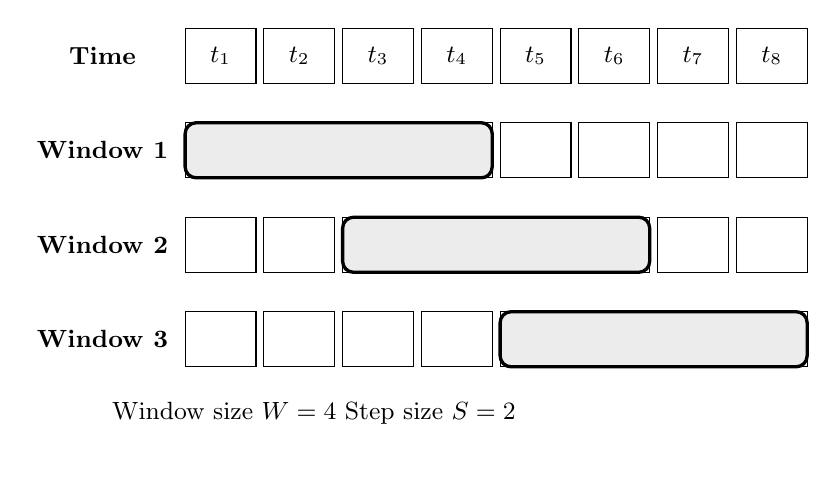
\begin{tikzpicture}[
        every node/.style={font=\small},
        cell/.style={draw, minimum width=0.9cm, minimum height=0.7cm, align=center},
        win/.style={draw, rounded corners, very thick,fill=gray!15}
    ]

        % Header row
        \node at (-1.5,0) {\textbf{Time}};
        \foreach \i/\t in {0/$t_1$,1/$t_2$,2/$t_3$,3/$t_4$,4/$t_5$,5/$t_6$,6/$t_7$,7/$t_8$} {
            \node[cell] (h\i) at (\i,0) {\t};
        }

        % Row 1
        \node at (-1.5,-1.2) {\textbf{Window 1}};
        \foreach \i in {0,...,7} {
            \node[cell] (a\i) at (\i,-1.2) {};
        }
        \draw[win] (-0.45,-1.55) rectangle (3.45,-0.85);

        % Row 2
        \node at (-1.5,-2.4) {\textbf{Window 2}};
        \foreach \i in {0,...,7} {
            \node[cell] (b\i) at (\i,-2.4) {};
        }
        \draw[win] (1.55,-2.75) rectangle (5.45,-2.05);

        % Row 3
        \node at (-1.5,-3.6) {\textbf{Window 3}};
        \foreach \i in {0,...,7} {
            \node[cell] (c\i) at (\i,-3.6) {};
        }
        \draw[win] (3.55,-3.95) rectangle (7.45,-3.25);

        % Note
        \node[align=center, anchor=west] at (-1.5,-4.7) {Window size $W = 4$  Step size $S = 2$\\};

    \end{tikzpicture}
    \caption{Ví dụ về cơ chế sliding window trên chuỗi dữ liệu thời gian thực}
    \label{fig:sliding-window}
\end{figure}
    Trong Hình~\ref{fig:sliding-window}, mỗi cửa sổ chứa một số lượng điểm dữ liệu cố định, được xác định bởi kích thước cửa sổ $W$. Sau mỗi lần xử lý, cửa sổ được dịch chuyển thêm một khoảng $S$, gọi là bước trượt. Việc lựa chọn $W$ và $S$ ảnh hưởng trực tiếp đến khả năng nắm bắt xu hướng dữ liệu, độ nhạy của hệ thống và chi phí tính toán.
    \subsubsection*{Chuẩn hóa Z-score động (Dynamic Z-score Normalization)}

    Trong không gian đặc trưng đa biến, các chỉ số hệ thống thường vận hành trên những thang đo và biên độ hoàn toàn khác biệt (ví dụ: mức sử dụng CPU giới hạn từ $0-100\%$, trong khi băng thông mạng có thể dao động tới hàng gigabyte). Sự chênh lệch phi tuyến tính này, nếu được đưa trực tiếp vào mạng nơ-ron, sẽ lập tức gây ra hiện tượng lấn át trọng số và làm quá trình hội tụ gradient bị chệch hướng. Do đó, việc đồng nhất hóa không gian biểu diễn là bước tiền xử lý bắt buộc, giúp mô hình tập trung học được bản chất tương quan giữa các biến thay vì bị nhiễu bởi độ lớn vật lý của con số.

    \textbf{Kỹ thuật chuẩn hóa Z-score} giải quyết bài toán này bằng cách tịnh tiến và thu phóng toàn bộ các biến số về chung một hệ quy chiếu. Về mặt toán học, phép biến đổi này ép mọi phân phối dữ liệu về dạng chuẩn với giá trị trung bình $\mu = 0$ và độ lệch chuẩn $\sigma = 1$. Đối với một điểm dữ liệu $x$, giá trị chuẩn hóa $z$ được tính toán theo phương trình:
    $$z = \frac{x - \mu}{\sigma}$$
    Trong môi trường dữ liệu luồng, giá trị trung bình $\mu$ và độ lệch chuẩn $\sigma$ thường được tính toán động dựa trên các giá trị bên trong Cửa sổ trượt hiện tại, giúp dữ liệu luôn giữ được tính ổn định ngay cả khi hệ thống thay đổi hành vi hoạt động.
    % \item \textbf{Dữ liệu chuỗi thời gian }\\
    % Trong bối cảnh giám sát hệ thống, các luồng thông tin thường được ghi nhận tại các khoảng thời gian đều đặn, tạo thành chuỗi thời gian. Chuỗi thời gian là một tập hợp các quan sát được sắp xếp theo trình tự thời gian xảy ra của chúng.
    
    % Đặc biệt, khi hệ thống cần giám sát nhiều thông số đồng thời (ví dụ: mức sử dụng CPU, dung lượng RAM khả dụng, tốc độ đọc/ghi của ổ cứng, lưu lượng mạng), dữ liệu được gọi là chuỗi thời gian đa biến (Multivariate Time-series).
    % Giả sử hệ thống giám sát $d$ chỉ số khác nhau. Tại mỗi bước thời gian $t$, trạng thái của hệ thống được biểu diễn bằng một véc-tơ $d$ chiều:
    %  $$X_t = [x_{1,t}, x_{2,t}, \dots, x_{d,t}]^T \in \mathbb{R}^d$$
    %  Khi đó, một dòng dữ liệu chuỗi thời gian đa biến từ thời điểm $1$ đến $t$ là một ma trận:
    %  $$X_{1:t} = [X_1, X_2, \dots, X_t]$$
    %  Việc phân tích chuỗi thời gian đa biến phức tạp hơn nhiều so với chuỗi đơn biến vì các thuật toán không chỉ phải nắm bắt sự phụ thuộc theo thời gian của từng biến riêng lẻ, mà còn phải mô hình hóa sự tương quan chéo giữa các biến với nhau tại cùng một thời điểm. Ví dụ, sự tăng đột biến của CPU có thể là bình thường nếu bộ nhớ RAM cũng phản ánh một khối lượng công việc tương ứng, nhưng sẽ là bất thường nếu các thông số khác không có sự thay đổi logic.

\subsection{Bài toán phát hiện bất thường trên chuỗi thời gian}
Sau khi dòng dữ liệu được tiền xử lý thành các trạng thái hữu hạn, hệ thống chuyển sang bước phân tích cốt lõi: phân loại trạng thái đó là bình thường hay bất thường. Phần này trình bày các định nghĩa nền tảng và phân tích rào cản thực tiễn mà các hệ thống giám sát hiện đại đang phải đối mặt.
\subsubsection{Định nghĩa và phân loại bất thường}
Về mặt hình thức, bài toán phát hiện bất thường trên chuỗi thời gian là một quá trình ánh xạ dữ liệu thành các nhãn phân loại. Cho trước một chuỗi quan sát $X = \{x_1, x_2, \dots, x_t\}$, mục tiêu là học một hàm $f(X)$ để gán nhãn $y_t \in \{0, 1\}$ cho thời điểm $t$, trong đó \textbf{$0$} đại diện cho trạng thái bình thường và \textbf{$1$} đại diện cho trạng thái bất thường.[1]

Dựa trên cấu trúc và biểu hiện của dữ liệu, các nghiên cứu nền tảng về khai phá dữ liệu thường phân loại bất thường thành ba nhóm chính:
\begin{itemize}
    \item \textbf{Bất thường điểm}: Xảy ra khi một điểm dữ liệu đơn lẻ có độ lệch cực đoan so với phân phối chung của phần còn lại của tập dữ liệu (ví dụ: mức sử dụng CPU đột ngột vọt lên 100\% trong một giây rồi lập tức hạ xuống). Dạng này có thể được phát hiện dễ dàng thông qua các ngưỡng thống kê truyền thống.

    \item \textbf{Bất thường tập hợp}: Là một chuỗi các điểm dữ liệu liên tiếp mà bản thân từng điểm đơn lẻ có thể không vượt ngưỡng nguy hiểm, nhưng khi xuất hiện cùng nhau lại tạo thành một mô hình hành vi sai lệch so với quy luật thông thường của hệ thống.

    \item \textbf{Bất thường ngữ cảnh}: Xảy ra khi một điểm hoặc một chuỗi dữ liệu được xem là bình thường trong một ngữ cảnh vận hành này, nhưng lại là bất thường khi đặt trong một ngữ cảnh khác. Ví dụ: Lưu lượng mạng tăng vọt lúc 02:00 AM là hành vi hợp lệ nếu hệ thống có lịch trình sao lưu dữ liệu, nhưng sẽ là dấu hiệu của một cuộc tấn công DDoS nếu diễn ra vào giờ hành chính mà không có sự kiện tương ứng nào được ghi nhận.
\end{itemize}

\subsubsection{Khoảng trống ngữ nghĩa}
Sự tồn tại của dạng bất thường ngữ cảnh đã bộc lộ giới hạn nghiêm trọng của các mô hình học máy và học sâu. Dù các kiến trúc mạng nơ-ron (như GNN, LSTM) thể hiện năng lực vượt trội trong việc tính toán khoảng cách không gian đa biến và phát hiện sự thay đổi phân phối, chúng bản chất vẫn là các cỗ máy tối ưu hóa toán học học trên dữ liệu số.

Tuy nhiên, các mô hình này hoàn toàn thiếu khả năng nhận thức về ngữ cảnh vận hành. Sự đứt gãy giữa con số và ngữ cảnh tạo ra một rào cản được gọi là Khoảng trống ngữ nghĩa (Semantic Gap). Khi một hệ thống giám sát chỉ dựa thuần túy vào thuật toán thống kê mà thiếu đi khả năng đọc hiểu các ngữ cảnh phi cấu trúc (như nhật ký hệ thống, lịch trình triển khai phần mềm), nó không thể phân biệt rạch ròi giữa một lỗi hệ thống thực sự và một sự thay đổi hành vi hợp lệ do con người chủ động can thiệp .

\begin{figure}[htbp]
    \centering
    \resizebox{0.95\textwidth}{!}{
    \begin{tikzpicture}[
        node distance=0.9cm and 1.5cm,
        box/.style={
            rectangle,
            draw,
            rounded corners,
            align=center,
            minimum width=3.2cm,
            minimum height=0.8cm,
            font=\small
        },
        decision/.style={
            diamond,
            draw,
            aspect=2.2,
            align=center,
            inner sep=1pt,
            font=\small
        },
        arrow/.style={-{Stealth}, thick}
    ]

        % Column titles
        \node[font=\small\bfseries] (title1) {Chỉ dùng metric};
        \node[font=\small\bfseries, right=5.2cm of title1] (title2) {Kết hợp thêm ngữ cảnh};

        % Left branch
        \node[box, below=0.5cm of title1] (metric) 
        {Metric bất thường\\CPU, Disk I/O, Latency tăng};

        \node[box, below=of metric] (detector) 
        {Mô hình phát hiện\\bất thường};

        \node[box, below=of detector] (alert) 
        {Cảnh báo được sinh ra};

        \node[box, below=of alert] (nogctx) 
        {Thiếu ngữ cảnh vận hành\\log, event, lịch triển khai};

        \node[box, below=of nogctx] (falsealert) 
        {Nguy cơ cảnh báo giả};

        \draw[arrow] (metric) -- (detector);
        \draw[arrow] (detector) -- (alert);
        \draw[arrow] (alert) -- (nogctx);
        \draw[arrow] (nogctx) -- (falsealert);

        % Right branch
        \node[box, below=0.5cm of title2] (metricctx) 
        {Metric bất thường\\+ Log + Event};

        \node[box, below=of metricctx] (analysis) 
        {Phân tích ngữ cảnh};

        \node[decision, below=1.0cm of analysis] (judge) 
        {Đánh giá\\cảnh báo};

        \node[box, below left=1.0cm and 0.7cm of judge] (valid) 
        {Cảnh báo hợp lệ};

        \node[box, below right=1.0cm and 0.7cm of judge] (fp) 
        {Loại bỏ\\cảnh báo giả};

        \draw[arrow] (metricctx) -- (analysis);
        \draw[arrow] (analysis) -- (judge);
        \draw[arrow] (judge) -- (valid);
        \draw[arrow] (judge) -- (fp);

    \end{tikzpicture}
    }
    \vspace{0.5cm}
    \caption{Khoảng trống ngữ nghĩa giữa bất thường định lượng và ngữ cảnh vận hành}
    \label{fig:semantic-gap}
\end{figure}
\subsubsection{Hiện tượng Quá tải cảnh báo}
Hệ quả trực tiếp của Khoảng trống ngữ nghĩa trong môi trường vận hành thực tế là sự gia tăng không kiểm soát của tỷ lệ báo động giả. Khi hệ thống liên tục phát đi cảnh báo đối với các sự kiện mang tính quy luật hoặc có thể giải thích được bằng lịch trình công việc, nó sẽ dẫn đến một hội chứng tâm lý và quy trình được gọi là Quá tải cảnh báo (Alert Fatigue) .

Các khảo sát thực nghiệm chỉ ra rằng việc phải tiếp nhận và xử lý hàng trăm cảnh báo "rác" mỗi ngày làm suy giảm nghiêm trọng sự nhạy cảm của đội ngũ vận hành. Điều này dẫn đến xu hướng phản ứng chậm trễ hoặc bỏ qua các thông báo, tạo ra rủi ro bỏ lọt những sự cố thực sự đang chìm lấp trong các cảnh báo giả. Do đó, việc thiết kế một cơ chế có khả năng thu hẹp khoảng trống ngữ nghĩa để chắt lọc cảnh báo cũng như việc ứng dụng các Mô hình Ngôn ngữ Lớn không chỉ là một bài toán tối ưu độ chính xác thuật toán, mà còn là yếu tố sống còn để đảm bảo tính khả dụng của quy trình giám sát AIOps.

\subsection{Các phương pháp phát hiện cơ sở}
Để xử lý khối lượng dữ liệu khổng lồ sinh ra từ luồng thời gian thực, hệ thống giám sát cần một mô hình cơ sở có khả năng tính toán tốc độ cao. Các mô hình sẽ đảm nhiệm vai trò này được gọi chung là các bộ phát hiện cơ sở. Phần này phân tích các phương pháp phân loại dữ liệu số phổ biến và chỉ ra những giới hạn của chúng trước bài toán ngữ cảnh.
\subsubsection{Các phương pháp thống kê và học máy truyền thống}
Lợi thế của nhóm phương pháp này nằm ở độ phức tạp tính toán thấp và khả năng hoạt động mà không đòi hỏi tài nguyên phần cứng chuyên dụng. Trong các hệ thống giám sát dòng dữ liệu, chúng đóng vai trò là hàng rào lọc nhiễu sơ cấp, giúp chặn đứng các dạng bất thường điểm rõ rệt nhất. Nhóm này được chia thành hai hướng tiếp cận chính:
\subsubsection*{Nhóm phương pháp dựa trên thống kê}
Các phương pháp thống kê vận hành dựa trên một giả định cốt lõi: dữ liệu bình thường của hệ thống tuân theo một phân phối xác suất có thể lập mô hình được.
\begin{itemize}[label=--]
    \item Đối với các hệ thống có tính chu kỳ, mô hình ARIMA thường được sử dụng. Thuật toán này phân tích chuỗi dữ liệu lịch sử để dự báo giá trị tiếp theo. Bất thường được xác định khi phần dư, tức sai số giữa giá trị dự báo và giá trị thực tế đo được vượt quá một ngưỡng độ tin cậy nhất định.
    \item Đối với các thuật toán giám sát động, các phép kiểm định độ lệch chuẩn (Z-score test) hoặc kiểm định giả thuyết được áp dụng để đánh giá xác suất xuất hiện của một điểm dữ liệu mới. Nếu xác suất này cực kỳ thấp so với phân phối chung, điểm đó bị gắn cờ cảnh báo.
\end{itemize}
\subsubsection*{Nhóm thuật toán học máy Decision Boundary}
Thay vì cố gắng lập mô hình phân phối xác suất của toàn bộ dữ liệu, các phương pháp học máy truyền thống tập trung vào việc khoanh vùng hoặc cô lập các điểm dữ liệu dị biệt trong không gian đặc trưng.
\begin{itemize}[label=--]
    \item \textbf{Isolation Forest}: Đây là một trong những thuật toán hiệu quả nhất cho dữ liệu dòng. Thay vì đi tìm "điểm bình thường", thuật toán này chủ động xây dựng các cây quyết định ngẫu nhiên để "cô lập" các điểm dữ liệu. Do các điểm bất thường có số lượng ít và giá trị chênh lệch lớn, chúng sẽ bị cô lập ở các nút rất gần gốc của cây phân lập. Quá trình này có độ phức tạp thuật toán cực thấp, rất lý tưởng cho môi trường thời gian thực.
    \item \textbf{One-Class SVM}: Thuật toán này tìm cách vẽ một hyperplane bao quanh toàn bộ tập dữ liệu bình thường trong không gian nhiều chiều. Những điểm dữ liệu rơi ra bên ngoài biên giới của hyperplane này sẽ bị phân loại là lỗi hệ thống.
\end{itemize}

Nhờ sự đơn giản về mặt toán học, nhóm thuật toán này thực thi với tốc độ cao, tiêu tốn rất ít bộ nhớ và hoàn toàn phù hợp để làm bộ lọc ban đầu (loại bỏ từ 80\% đến 90\% dữ liệu bình thường).

Tuy nhiên, rào cản chí mạng của nhóm phương pháp này khi áp dụng vào thực tế là chiều dữ liệu  Khi hệ thống giám sát mở rộng lên hàng trăm chỉ số (CPU, RAM, Disk I/O, Network), các phương pháp thống kê buộc phải phân tích từng biến một cách độc lập, bỏ qua hoàn toàn sự đồng biến động giữa chúng. Tương tự, One-Class SVM hay Isolation Forest chỉ hoạt động tốt trên không gian dữ liệu có số chiều nhỏ và biểu diễn được các phép đo tuyến tính. Chúng không hoạt động tốt trước các lỗi hệ thống phức tạp phát sinh từ sự tương tác phi tuyến tính giữa các biến số (ví dụ: CPU tăng nhẹ kết hợp với độ trễ phản hồi Database kéo dài). Sự thiếu hụt năng lực phân tích đa biến này đòi hỏi hệ thống phải có một lớp thuật toán sâu hơn để giải quyết, đó chính là các mô hình học sâu.

\subsubsection{Các mô hình học sâu cho chuỗi thời gian}
Để xử lý dữ liệu có nhiều chiều và các mối quan hệ phức tạp giữa các biến, các mô hình học sâu ngày nay thường được dùng làm nền tảng cho hệ thống phát hiện bất thường. Thay vì phải tự tay xây dựng đặc trưng từ dữ liệu, các mô hình này có thể tự học cách biểu diễn dữ liệu từ dạng thô, giúp hệ thống hiểu rõ hơn cách các tín hiệu thay đổi theo thời gian và cách chúng liên hệ với nhau.
\subsubsection*{Khai thác mối quan hệ theo thời gian}
Trong nhiều trường hợp, bất thường không xuất hiện ngay lập tức mà tích lũy dần theo thời gian. Ví dụ, một hệ thống có thể hoạt động bình thường trong thời gian ngắn, nhưng sau đó bắt đầu lệch khỏi trạng thái ổn định do lỗi tích tụ. Vì vậy, mô hình cần có khả năng “nhìn lại quá khứ” để hiểu được xu hướng thay đổi của dữ liệu.
Một số kiến trúc thường được sử dụng:
\begin{itemize}[label=--]
    \item \textbf{Mạng LSTM (Long Short-Term Memory)}: Khác với mạng feed-forward thông thường, LSTM sở hữu các vòng lặp phản hồi và cơ chế cổng. Nhờ đó, nó giải quyết được hiện tượng triệt tiêu đạo hàm (vanishing gradient), cho phép mô hình lưu giữ trạng thái của hệ thống qua hàng trăm bước thời gian trong quá khứ để dự đoán hành vi tương lai. LSTM phù hợp với các trường hợp như: xu hướng tăng/giảm chậm, lỗi tích lũy theo thời gian và các bất thường dạng chuỗi.
    \item \textbf{Mô hình Transformer}: kiến trúc Transformer dựa trên cơ chế Self-Attention được ứng dụng mạnh mẽ vào chuỗi thời gian. Thay vì xử lý tuần tự, cơ chế này tính toán trọng số tương quan giữa điểm dữ liệu hiện tại với mọi điểm dữ liệu trong cửa sổ lịch sử cùng lúc. Điều này giúp mô hình bắt được các phụ thuộc chu kỳ dài hạn mà LSTM có thể bỏ sót.
\end{itemize}

\subsubsection*{Khai thác mối quan hệ giữa nhiều biến}
Trong thực tế, các chỉ số hệ thống thường có xu hướng biến động cùng nhau. Ví dụ, tải CPU tăng có thể đi kèm với lưu lượng mạng tăng trong các hệ thống xử lý yêu cầu, hoặc hoạt động đọc/ghi đĩa cao thường liên quan đến các tiến trình xử lý dữ liệu. Tuy nhiên, các mối quan hệ này không mang tính tuyệt đối và có thể thay đổi tùy theo ngữ cảnh vận hành. Do đó, việc chỉ dựa trên giá trị riêng lẻ của từng chỉ số là không đủ để xác định bất thường, mà cần xem xét đồng thời mối quan hệ giữa các biến và bối cảnh hệ thống.

Để giải quyết vấn đề này, mạng nơ-ron đồ thị (Graph Neural Network - GNN) được sử dụng nhằm mô hình hóa hệ thống dưới dạng đồ thị $\textbf{G = (V, E)}$, trong đó mỗi nút đại diện cho một biến và các cạnh biểu diễn mức độ liên kết giữa chúng. Thông qua cơ chế lan truyền thông tin giữa các nút, mô hình có thể cập nhật trạng thái của từng biến dựa trên thông tin tổng hợp từ các biến liên quan.

Cách tiếp cận này cho phép phát hiện các bất thường xuất phát từ sự phá vỡ mối quan hệ giữa các biến, ngay cả khi giá trị của từng biến riêng lẻ vẫn nằm trong ngưỡng bình thường. Chẳng hạn, nếu CPU và Network thường tăng cùng nhau, nhưng tại thời điểm $t$, CPU vọt lên 90\% trong khi Network rớt xuống 0\%, GNN sẽ ngay lập tức bắt được sự bất thường này, ngay cả khi mức 90\% của CPU chưa hề chạm đến ngưỡng báo động cứng.

\subsection{Mô hình Ngôn ngữ Lớn trong Giám sát Hệ thống}
\subsubsection{Tổng quan về mô hình ngôn ngữ lớn}
\textbf{Mô hình ngôn ngữ lớn} là một lớp hệ thống trí tuệ nhân tạo hiện đại được xây dựng chủ yếu trên kiến trúc Transformer. Các mô hình này được huấn luyện trên tập dữ liệu văn bản rất lớn, cho phép chúng học được cách biểu diễn và xử lý ngôn ngữ tự nhiên ở mức độ sâu. Thay vì chỉ thực hiện các phép ánh xạ đơn giản từ dữ liệu đầu vào sang nhãn đầu ra như nhiều phương pháp học máy truyền thống, mô hình ngôn ngữ lớn có khả năng nắm bắt ý nghĩa của văn bản, suy luận dựa trên ngữ cảnh và tổng hợp thông tin từ nhiều nguồn khác nhau.

Trong bài toán giám sát hệ thống, điểm mạnh quan trọng của các mô hình này nằm ở khả năng xử lý thông tin mang tính ngữ nghĩa. Các phương pháp truyền thống thường dựa vào ngưỡng hoặc các quy tắc cố định để phát hiện bất thường, do đó dễ tạo ra nhiều cảnh báo không cần thiết khi thiếu thông tin bối cảnh. Ngược lại, mô hình ngôn ngữ lớn có thể kết hợp dữ liệu định lượng (như chỉ số CPU, RAM) với thông tin định tính (như nhật ký hệ thống, lịch vận hành) để đưa ra đánh giá chính xác hơn.

Ví dụ, khi hệ thống ghi nhận mức sử dụng CPU tăng đột biến, các phương pháp đơn giản có thể coi đây là dấu hiệu bất thường. Tuy nhiên, nếu đồng thời tồn tại thông tin cho thấy hệ thống đang thực hiện một tác vụ đã được lên lịch, mô hình ngôn ngữ lớn có thể suy luận rằng sự thay đổi này là hợp lý trong bối cảnh hiện tại. Khả năng liên kết giữa dữ liệu và ngữ cảnh như vậy giúp giảm đáng kể số lượng cảnh báo sai và nâng cao độ tin cậy của hệ thống giám sát.

Nhờ những đặc điểm này, mô hình ngôn ngữ lớn thường được sử dụng như một lớp xử lý bổ sung trong các kiến trúc giám sát hiện đại, đóng vai trò phân tích ngữ nghĩa và hỗ trợ ra quyết định, thay vì thay thế hoàn toàn các mô hình phát hiện bất thường truyền thống.
\subsubsection{Hạn chế của LLM trong hệ thống thời gian thực}
Mặc dù các mô hình ngôn ngữ lớn thể hiện khả năng suy luận mạnh mẽ, chúng không phù hợp để xử lý trực tiếp toàn bộ luồng dữ liệu trong môi trường thời gian thực. Điều này xuất phát từ một số ràng buộc kỹ thuật cơ bản:

\begin{itemize}[label=--]
    \item \textbf{Độ trễ suy luận}: Độ trễ là một trong những hạn chế lớn nhất khi triển khai LLM trong hệ thống thời gian thực. Các mô hình phát hiện bất thường truyền thống như GNN hoặc Isolation Forest có thể xử lý dữ liệu trong thời gian rất ngắn, thường chỉ ở mức mili-giây. Trong khi đó, một lần gọi LLM để sinh phản hồi có thể mất từ vài giây trở lên. Mức độ trễ này khiến LLM không đáp ứng được yêu cầu phản ứng tức thời của các hệ thống giám sát liên tục.
    \item \textbf{Chi phí vận hành}: Chi phí là yếu tố quan trọng khi áp dụng LLM vào các hệ thống xử lý dữ liệu quy mô lớn. Các mô hình thương mại thường tính phí dựa trên số lượng token của cả đầu vào và đầu ra. Khi dữ liệu được sinh ra liên tục với tần suất cao, việc gọi LLM cho từng sự kiện sẽ làm chi phí tăng nhanh và khó kiểm soát, đặc biệt trong các hệ thống cần hoạt động dài hạn.
    \item \textbf{Giới hạn ngữ cảnh}: LLM bị giới hạn bởi kích thước cửa sổ ngữ cảnh trong mỗi lần xử lý. Trong khi đó, dữ liệu giám sát thường bao gồm số lượng lớn các bản ghi và chỉ số theo thời gian. Việc đưa toàn bộ dữ liệu này vào một lần xử lý có thể vượt quá khả năng của mô hình, dẫn đến việc bỏ sót thông tin hoặc làm giảm độ chính xác của kết quả.
    \item \textbf{Hệ quả đối với thiết kế hệ thống}: Từ các hạn chế trên, có thể rút ra một nguyên tắc thiết kế quan trọng: LLM không nên được sử dụng để xử lý toàn bộ dữ liệu đầu vào. Thay vào đó, LLM nên được đặt ở giai đoạn sau của hệ thống, nơi chỉ xử lý một tập nhỏ các sự kiện đã được sàng lọc trước bởi các mô hình nhẹ và có độ trễ thấp. Cách tiếp cận này cho phép tận dụng khả năng suy luận của LLM, đồng thời đảm bảo hiệu năng và chi phí vận hành của toàn hệ thống.
\end{itemize}

\subsubsection{Kỹ thuật Prompt và Ràng buộc Đầu ra Có Cấu trúc}
Bản chất của LLM là một mô hình sinh văn bản xác suất: với cùng một câu hỏi, mô hình có thể trả lời theo vô số cách khác nhau, với độ dài, cấu trúc và phong cách hoàn toàn không nhất quán. Trong môi trường chatbot hay hỗ trợ sáng tạo, đặc điểm này là một lợi thế. Tuy nhiên, khi LLM được tích hợp vào một hệ thống tự động – nơi đầu ra của nó phải được phân tích cú pháp bởi code và dẫn đến các hành động cụ thể như gửi cảnh báo, ghi log hay kích hoạt quy trình xử lý sự cố – sự không nhất quán này trở thành một rủi ro nghiêm trọng.

\textbf{Prompt Engineering }là tập hợp các phương pháp thiết kế câu lệnh đầu vào một cách có chủ đích, nhằm định hướng hành vi của LLM sao cho phù hợp với yêu cầu kỹ thuật của hệ thống. Đây không đơn thuần là việc "viết câu hỏi rõ ràng hơn", mà là một kỷ luật kỹ thuật với các nguyên tắc, kỹ thuật và mẫu thiết kế riêng biệt.

\subsubsection*{Kiến trúc Prompt trong hệ thống giám sát}

Một prompt hoàn chỉnh gửi đến LLM trong hệ thống giám sát thường được cấu thành từ ba thành phần riêng biệt, đóng các vai trò khác nhau:
\begin{itemize}
    \item \textbf{System Prompt}: là phần được định nghĩa cố định bởi nhà phát triển và không thay đổi giữa các lần gọi. Thành phần này thiết lập vai trò và cách hành xử của mô hình trong toàn bộ phiên làm việc. Cụ thể, System Prompt quy định nhiệm vụ cần thực hiện, nguyên tắc suy luận cần tuân theo, cũng như định dạng đầu ra bắt buộc. Trong bài toán giám sát hệ thống, System Prompt thường hướng dẫn mô hình ưu tiên kiểm tra các nguyên nhân hợp lệ đã biết, chẳng hạn như các tác vụ định kỳ hoặc sự kiện có kế hoạch, trước khi kết luận một sự cố. Đồng thời, nó cũng ràng buộc mô hình phải trả về kết quả theo một cấu trúc định dạng xác định (ví dụ: JSON), nhằm đảm bảo tính nhất quán và khả năng tích hợp với các thành phần khác trong hệ thống. Ví dụ: 
    \begin{mdframed}[
  backgroundcolor=gray!10,
  linecolor=gray!60,
  linewidth=1pt,
  innerleftmargin=10pt,
  innerrightmargin=10pt
]
\small
\textbf{System Prompt:}\\[4pt]
\textit{``You are an IT infrastructure incident analysis system. Your task is to evaluate the severity of an alert based on the provided system metrics and logs. When performing the analysis, prioritize identifying known legitimate causes (such as scheduled tasks or planned events) before concluding that the situation is a real incident. You MUST respond strictly in the following JSON format and must not include any additional text outside of that JSON.``}
\end{mdframed}
\item \textbf{Context Block}: là phần nội dung động, thay đổi theo từng sự kiện. Đây là nơi hệ thống RAG chèn vào các tài liệu tham chiếu đã truy xuất được. Phần này bao gồm nhật ký liên quan, lịch trình tác vụ, hoặc lịch sử sự cố tương tự trong quá khứ. Thành phần này đóng vai trò cung cấp "bộ nhớ ngắn hạn" tình huống cho LLM, bù đắp cho việc mô hình không có thông tin nội bộ sẵn có sau khi huấn luyện.
\item \textbf{Query Block}: là phần mô tả trực tiếp sự kiện cần được đánh giá. Nội dung này thường được sinh ra từ tầng phát hiện bất thường và được chuẩn hóa theo một khuôn dạng nhất định. Thông tin trong Query Block có thể bao gồm các chỉ số hệ thống tại thời điểm xảy ra sự kiện, thời gian duy trì, cũng như các tiến trình hoặc thành phần liên quan.  Ví dụ: "Sự kiện: CPU Server-01 đạt 94\% lúc 02:17. Thời gian duy trì: 18 phút. Các tiến trình có tải cao nhất: mysqldump (87\%), rsync (6\%)."
\end{itemize}
Ba thành phần này được ghép nối theo thứ tự cố định và gửi đến LLM trong một lần gọi duy nhất, tạo thành một prompt hoàn chỉnh, đầy đủ ngữ cảnh và có cấu trúc rõ ràng.

\subsubsection*{Ràng buộc đầu ra có cấu trúc}
Ràng buộc định dạng \textbf{JSON} là một kỹ thuật quan trọng nhằm chuẩn hóa đầu ra của mô hình ngôn ngữ lớn trong các hệ thống tự động. Tuy nhiên, việc chỉ yêu cầu mô hình “trả về JSON” là chưa đủ để đảm bảo tính ổn định và nhất quán trong thực tế. Do đó, một số kỹ thuật bổ sung thường được áp dụng nhằm kiểm soát hành vi của mô hình.

Trước hết, cần định nghĩa rõ ràng schema đầu ra ngay trong \textbf{System Prompt}. Thay vì mô tả chung chung, mỗi trường dữ liệu cần được chỉ định cụ thể về tên, kiểu giá trị và ý nghĩa. Điều này giúp giảm thiểu sai lệch trong quá trình sinh kết quả và đảm bảo đầu ra có thể được xử lý tự động bởi các thành phần phía sau.

\textbf{Ví dụ}, một schema cho bài toán phân loại cảnh báo có thể được định nghĩa như sau:
\begin{table}[H]
\centering
\begin{tcolorbox}[
    colback=gray!5,       % Màu nền hộp (xám nhạt 5%)
    colframe=blue!50!black, % Màu viền hộp (xanh đen)
    arc=4mm,              % Độ bo góc
    fonttitle=\small\bfseries,
    halign title=center,  % Căn giữa tiêu đề
    width=0.85\textwidth  % Độ rộng của hộp so với trang giấy
]
\begin{lstlisting}[basicstyle=\small\ttfamily, columns=fullflexible, keepspaces=true]
{
  "label": "true_alert | false_positive | uncertain",
  "severity": "P1 | P2 | P3 | none",
  "confidence": 0.0,
  "evidence": ["doc_id_1", "doc_id_2"],
  "reason": "short explanation",
  "recommended_action": "short action"
}
\end{lstlisting}
\end{tcolorbox}
\caption{Định dạng cấu trúc đầu ra từ mô hình ngôn ngữ lớn}
\label{tab:llm_json_schema}
\end{table}
\textbf{\textit{Lưu ý}}: Schema trong bảng trên phản ánh định dạng đầu ra thực tế được sử dụng trong thực nghiệm (xem mục 4.3.2). Trường label sử dụng ba nhãn thay vì phân loại mức độ nghiêm trọng, vì mục tiêu của tầng LLM-as-a-Judge là quyết định có nên định tuyến cảnh báo hay không, chứ không phải phân loại mức P1/P2. Trường evidence tham chiếu đến doc\_id của các log/trace đã được RAG truy xuất, tạo ra khả năng kiểm tra ngược lại bằng chứng.

Bên cạnh đó, kỹ thuật \textbf{few-shot prompting} thường được sử dụng bằng cách cung cấp một số cặp ví dụ đầu vào–đầu ra ngay trong prompt. Các ví dụ này giúp mô hình học được cách biểu diễn kết quả một cách trực quan, từ đó cải thiện đáng kể tính nhất quán so với việc chỉ đưa ra mô tả bằng lời.

Cuối cùng, đối với các tình huống phức tạp, có thể áp dụng phương pháp hướng dẫn suy luận theo từng bước. Cụ thể, schema đầu ra có thể được mở rộng với một trường như \textit{reasoning\_steps}, cho phép mô hình trình bày các bước lập luận trước khi đưa ra kết luận cuối cùng. Cách tiếp cận này không chỉ nâng cao chất lượng dự đoán mà còn tăng khả năng giải thích và kiểm tra lại kết quả trong quá trình vận hành hệ thống.

\subsubsection*{Đảm bảo tính hợp lệ và độ tin cậy của đầu ra LLM}
Mặc dù prompt và schema đầu ra được thiết kế cẩn thận, trong môi trường triển khai thực tế, mô hình ngôn ngữ lớn vẫn có thể sinh ra các kết quả không hợp lệ. Các lỗi phổ biến bao gồm sai cú pháp JSON, thiếu các trường bắt buộc, hoặc giá trị không nằm trong miền hợp lệ đã định nghĩa. Do đó, việc xây dựng cơ chế kiểm soát và xử lý lỗi là một yêu cầu thiết yếu nhằm đảm bảo tính ổn định của toàn hệ thống.

Một phương pháp cơ bản là triển khai lớp validation ngay sau khi nhận phản hồi từ LLM. Lớp này thực hiện đối chiếu đầu ra với schema đã định nghĩa, bao gồm kiểm tra cấu trúc, kiểu dữ liệu và giá trị hợp lệ của từng trường. Chỉ khi đầu ra vượt qua bước kiểm tra này, hệ thống mới tiếp tục các bước xử lý tiếp theo. Ngược lại, nếu phát hiện sai lệch, hệ thống có thể kích hoạt cơ chế gọi lại LLM kèm theo thông tin phản hồi về lỗi cụ thể. Cách tiếp cận này, thường được gọi là self-correction prompting, cho phép mô hình tự điều chỉnh đầu ra dựa trên phản hồi, từ đó cải thiện đáng kể tỷ lệ trả về kết quả hợp lệ.

Ngoài ra, các nền tảng API hiện đại cung cấp cơ chế ràng buộc cấu trúc đầu ra ngay từ quá trình sinh token. Cụ thể, thông qua các tính năng như \textit{Structured Outputs} hoặc \textit{Function Calling}, nhà phát triển có thể khai báo trực tiếp schema JSON ở cấp độ API. Khi đó, mô hình sẽ bị giới hạn trong việc sinh ra các token phù hợp với cấu trúc đã định nghĩa, giúp giảm thiểu hoặc loại bỏ hoàn toàn các lỗi liên quan đến định dạng. Đây là giải pháp có độ tin cậy cao và đặc biệt phù hợp với các hệ thống yêu cầu tính chính xác và ổn định trong môi trường sản xuất.

Tổng thể, việc kết hợp giữa kiểm tra hậu xử lý và ràng buộc ở cấp độ sinh token tạo thành một cơ chế bảo vệ nhiều lớp, giúp nâng cao đáng kể tính bền vững và khả năng vận hành liên tục của hệ thống sử dụng LLM.
\subsubsection*{Vai trò của Prompt Engineering trong kiến trúc tổng thể}

Trong bối cảnh hệ thống giám sát tích hợp LLM, Prompt Engineering không chỉ là một kỹ thuật hỗ trợ mà đóng vai trò như một lớp giao tiếp trung tâm giữa logic nghiệp vụ và khả năng suy luận của mô hình. Thông qua prompt, các yêu cầu nghiệp vụ được chuyển hóa thành dạng mà LLM có thể hiểu và xử lý, đồng thời kiểm soát cách thức mô hình đưa ra kết luận và biểu diễn kết quả.

Chất lượng của prompt ảnh hưởng trực tiếp đến độ chính xác, tính nhất quán và khả năng tích hợp của hệ thống. Một System Prompt được thiết kế tốt có thể định hướng mô hình tuân thủ các quy tắc suy luận cụ thể, ưu tiên các yếu tố ngữ cảnh quan trọng và đảm bảo đầu ra phù hợp với định dạng yêu cầu. Ngược lại, một prompt thiếu chặt chẽ có thể dẫn đến các kết quả không ổn định, làm suy giảm độ tin cậy của toàn bộ pipeline xử lý.

Do đó, trong các hệ thống thực tế, Prompt Engineering cần được xem như một thành phần kỹ thuật chính thức. Các prompt nên được quản lý phiên bản tương tự như mã nguồn, cho phép theo dõi thay đổi và quay lại các phiên bản ổn định khi cần thiết. Bên cạnh đó, việc kiểm thử hồi quy cũng đóng vai trò quan trọng nhằm đảm bảo rằng các thay đổi trong prompt không làm suy giảm hiệu năng trên các tình huống đã được kiểm chứng trước đó. Cuối cùng, prompt cần được tinh chỉnh liên tục dựa trên dữ liệu vận hành thực tế, giúp hệ thống thích nghi với các kịch bản mới và cải thiện hiệu quả theo thời gian.

Cách tiếp cận này giúp đảm bảo rằng LLM không chỉ là một thành phần bổ sung, mà trở thành một phần được kiểm soát chặt chẽ và có thể dự đoán trong kiến trúc tổng thể của hệ thống giám sát.
\subsection{Triển khai LLM cục bộ và API fallback}
Trong các hệ thống sử dụng LLM, mô hình có thể được triển khai theo hai hướng chính: gọi mô hình thông qua API bên ngoài hoặc chạy mô hình cục bộ trên máy chủ nội bộ. Cách gọi API thường cho chất lượng suy luận ổn định hơn và dễ tích hợp, nhưng phát sinh chi phí, phụ thuộc vào kết nối mạng, quota và độ trễ của nhà cung cấp. Ngược lại, mô hình cục bộ giúp giảm chi phí gọi mô hình và hạn chế việc gửi dữ liệu vận hành ra bên ngoài, nhưng thường bị giới hạn bởi tài nguyên phần cứng và chất lượng suy luận của các mô hình nhỏ.

Để cân bằng giữa chi phí và độ tin cậy, một chiến lược thường được sử dụng là local-first with API fallback. Theo chiến lược này, hệ thống ưu tiên gọi mô hình cục bộ để xử lý các cảnh báo đơn giản. Nếu kết quả cục bộ không hợp lệ, có độ tin cậy thấp, phân loại là\textit{ uncertain}, hoặc \textit{cảnh báo có mức độ bất thường cao}, hệ thống sẽ gọi \textit{mô hình API} mạnh hơn để thẩm định lại. Cách tiếp cận này giúp giảm số lần gọi API trong khi vẫn giữ một cơ chế dự phòng cho các trường hợp khó.

Trong bài toán giám sát thời gian thực, chiến lược \textit{local-first} phù hợp với vai trò LLM-as-a-Judge vì không phải mọi cảnh báo đều cần được gửi đến mô hình API. Các cảnh báo có ngữ cảnh rõ ràng có thể được xử lý bởi mô hình local, trong khi các trường hợp phức tạp được chuyển sang \textit{API fallback}. Tuy nhiên, do mô hình local nhỏ có thể sinh đầu ra không ổn định, hệ thống cần ràng buộc đầu ra bằng JSON schema và có cơ chế kiểm tra hợp lệ trước khi đưa ra quyết định cuối cùng.
\subsection{Retrieval-Augmented Generation trong hệ thống giám sát}

\textbf{Retrieval-Augmented Generation (RAG)} là kỹ thuật kết hợp giữa mô hình ngôn ngữ lớn và một cơ chế truy xuất thông tin từ nguồn dữ liệu bên ngoài. Thay vì yêu cầu LLM chỉ dựa vào kiến thức đã học trong quá trình huấn luyện, hệ thống sẽ tìm kiếm các tài liệu hoặc bản ghi liên quan đến truy vấn hiện tại, sau đó đưa các thông tin này vào prompt như một phần ngữ cảnh bổ sung.

Trong bài toán giám sát hệ thống, nguồn dữ liệu truy xuất có thể bao gồm log, trace, sự kiện triển khai, lịch bảo trì hoặc tài liệu vận hành. Khi một mô hình phát hiện bất thường đánh dấu một cửa sổ metric là nghi vấn, RAG được sử dụng để truy xuất các log hoặc trace liên quan đến cùng khoảng thời gian, cùng service hoặc cùng node. Các thông tin này giúp LLM có thêm bằng chứng để đánh giá liệu cảnh báo là sự cố thật sự hay chỉ là biến động hợp lệ trong vận hành.

Việc sử dụng RAG là cần thiết vì metric thường chỉ phản ánh sự thay đổi định lượng của hệ thống, nhưng không giải thích được nguyên nhân phía sau sự thay đổi đó. Nếu chỉ đưa metric vào LLM, mô hình có thể thiếu ngữ cảnh để phân biệt giữa cảnh báo thật và cảnh báo giả. Ngược lại, nếu đưa toàn bộ log và trace vào LLM, hệ thống sẽ gặp vấn đề về giới hạn ngữ cảnh, độ trễ và chi phí xử lý. RAG đóng vai trò trung gian bằng cách chọn lọc một số lượng nhỏ các thông tin liên quan nhất, giúp LLM suy luận có căn cứ hơn trong khi vẫn kiểm soát được kích thước prompt.

Trong phạm vi nghiên cứu này, RAG không được sử dụng như một hệ thống hỏi đáp độc lập, mà là một thành phần hỗ trợ cho tầng LLM-as-a-Judge. Cụ thể, RAG nhận đầu vào là thông tin của cảnh báo ứng viên, bao gồm khoảng thời gian, service, node và các metric bất thường, sau đó truy xuất \textbf{top-k log/trace} liên quan. Các ngữ cảnh này được kết hợp với metric snapshot trong prompt để LLM đưa ra quyết định cuối cùng dưới dạng có cấu trúc.
\subsubsection*{Lựa chọn cơ chế truy xuất trong bài toán giám sát}
Trong thực tế triển khai, lựa chọn phương pháp truy xuất ảnh hưởng đáng kể đến chất lượng ngữ cảnh đưa vào LLM. Hai hướng chính thường được xem xét là truy xuất thuần ngữ nghĩa (semantic/vector search) và truy xuất từ khóa (BM25). Truy xuất ngữ nghĩa dựa trên độ tương đồng embedding phù hợp với trường hợp truy vấn và tài liệu có cách diễn đạt khác nhau nhưng cùng ý nghĩa. Truy xuất BM25 dựa trên tần suất từ khóa, phù hợp hơn khi log và trace chứa các định danh chính xác như tên service, tên pod, mã lỗi hoặc tên fault type.
Trong môi trường giám sát server/cloud, log và trace thường chứa các chuỗi định danh cụ thể — ví dụ \textit{cartservice, network\_delay, checkoutservice} — mà vector embedding có thể không bảo toàn tốt tính đặc trưng. Vì vậy, một chiến lược phổ biến là kết hợp cả hai: \textbf{hybrid retrieval} dùng \textbf{BM25} để đối sánh từ khóa chính xác và dùng semantic hashing để bổ sung độ phủ ngữ nghĩa, sau đó kết hợp điểm số từ hai nguồn cùng với metadata (thời gian, service, severity) để xếp hạng kết quả. Cách kết hợp này giúp tăng khả năng tìm thấy log lỗi liên quan ngay cả khi tên chính xác của service không xuất hiện trong truy vấn, đồng thời vẫn bắt được các sự kiện có cùng dấu hiệu bất thường nhưng dùng thuật ngữ khác nhau.
\subsection{Khung kiến trúc giám sát lai và cơ chế "LLM-as-a-Judge"}
\subsubsection{Định nghĩa cơ chế "LLM-as-a-Judge"}
\textbf{Khái niệm “LLM-as-a-Judge”} ban đầu được đề xuất trong bối cảnh đánh giá ngoại tuyến đầu ra của các mô hình học máy. Tuy nhiên, trong các hệ thống hiện đại, cơ chế này đã được mở rộng và tích hợp trực tiếp vào quy trình xử lý trực tuyến. Thay vì chỉ đóng vai trò đánh giá thụ động, mô hình ngôn ngữ lớn được thiết kế thông qua các cấu trúc prompt chặt chẽ để hoạt động như một bộ phân tích ngữ nghĩa ở giai đoạn cuối của pipeline.

Trong bài toán phát hiện bất thường trên dòng dữ liệu liên tục, LLM không trực tiếp xử lý toàn bộ dữ liệu đầu vào. Thay vào đó, khi một mô hình phát hiện bất thường ở tầng trước xác định một điểm ngoại lệ, hệ thống sẽ xây dựng một tập thông tin mô tả sự kiện và chuyển đến LLM để đánh giá. Tập thông tin này thường bao gồm: 
\begin{itemize}[label=--]
    \item \textbf{Chi tiết điểm ngoại lệ}: dấu thời gian, giá trị quan sát, giá trị dự đoán và ngưỡng bất thường
    \item \textbf{Bối cảnh dữ liệu lân cận}: các điểm dữ liệu trước và sau thời điểm xảy ra sự kiện
    \item \textbf{Các đặc trưng thống kê}: giá trị trung bình và độ lệch chuẩn của chuỗi dữ liệu trong các khoảng thời gian liên quan.
\end{itemize}
Dựa trên tập ngữ cảnh được cung cấp, LLM thực hiện hai chức năng chính và trả về kết quả dưới dạng JSON có cấu trúc:
\begin{itemize}[label=--]
    \item LLM thực hiện phân loại ngữ nghĩa trực tiếp trong luồng xử lý cảnh báo. Trong ứng dụng offline ban đầu, cơ chế "judge" được dùng để gán nhãn KEEP/REMOVE cho dữ liệu huấn luyện. Trong bài toán giám sát của đề tài này, cơ chế được điều chỉnh để đưa ra quyết định định tuyến trực tiếp đối với từng cảnh báo ứng viên. Cụ thể, LLM phân loại mỗi cảnh báo thành một trong ba nhãn:

    \begin{itemize}
        \item \textbf{True Alert}: cảnh báo có bằng chứng rõ ràng về sự cố thật, được định tuyến đến đội vận hành.
        \item \textbf{False Positive}: biến động metric được giải thích bởi ngữ cảnh vận hành hợp lệ (batch job, deployment, autoscaling...), bị loại bỏ.
        \item \textbf{Uncertain}: ngữ cảnh chưa đủ để kết luận, đưa vào hàng chờ manual review.
    \end{itemize}
Mỗi quyết định đi kèm với trường confidence (0.0–1.0), danh sách evidence tham chiếu đến các log/trace cụ thể đã được RAG truy xuất, và trường reason giải thích ngắn gọn căn cứ suy luận. Yêu cầu cung cấp evidence cụ thể là thiết yếu: một LLM không thể trả về \textbf{True Alert} nếu không chỉ ra được bằng chứng cụ thể nào từ log/trace hỗ trợ kết luận đó. Điều này giúp kiểm soát \textbf{False Positive} do LLM "đoán mò" khi thiếu ngữ cảnh.
    \item LLM cung cấp khả năng giải thích thông qua việc sinh ra các bước lập luận. Cơ chế này cho phép mô hình trình bày rõ ràng các yếu tố dẫn đến quyết định cuối cùng, từ đó khắc phục hạn chế “hộp đen” của các mô hình định lượng. Thay vì chỉ đưa ra kết luận, LLM mô phỏng quá trình phân tích của một kỹ sư hệ thống bằng cách liên kết các bằng chứng trong dữ liệu với các quy luật vận hành. Ví dụ, nếu chuỗi dữ liệu sau điểm bất thường không quay về mức trung bình ban đầu mà thiết lập một trạng thái ổn định mới, mô hình có thể suy luận rằng đây là dấu hiệu của một sự thay đổi dài hạn thay vì một lỗi tạm thời, từ đó đưa ra quyết định giữ lại sự kiện.
\end{itemize}
Nhìn chung, cơ chế “LLM-as-a-Judge” đóng vai trò cầu nối giữa các mô hình phát hiện định lượng và quá trình ra quyết định ở mức hệ thống. Bằng cách bổ sung khả năng suy luận ngữ nghĩa và giải thích, LLM giúp nâng cao độ chính xác, giảm thiểu cảnh báo sai và hỗ trợ quá trình học thích ứng trong các hệ thống giám sát thời gian thực.

\subsubsection{Kiến trúc giám sát lai hai tầng}
Để tích hợp cơ chế "Thẩm phán LLM" vào môi trường dữ liệu đổ về liên tục mà không làm hệ thống bị nghẽn hay tốn quá nhiều chi phí API, một Kiến trúc Lai hai tầng được thiết lập. Kiến trúc này hoạt động như một chiếc phễu lọc, phân bổ đúng công việc cho đúng công cụ:

\subsubsection*{Tầng 1 - Fast Scanning:}
Dòng dữ liệu metric liên tục chảy qua một mô hình phát hiện bất thường 
tốc độ cao. Mô hình ở tầng này thường thuộc nhóm thuật toán thống kê 
hoặc học máy nhẹ — những phương pháp có thể đưa ra quyết định trong 
thời gian mili-giây mà không đòi hỏi tài nguyên tính toán lớn. Nhiệm vụ 
của tầng này không phải là phán xét cuối cùng, mà là sàng lọc: loại bỏ 
phần lớn các cửa sổ dữ liệu hoàn toàn bình thường và chỉ giữ lại một tập 
nhỏ các cửa sổ có dấu hiệu đáng nghi để chuyển xuống tầng tiếp theo. 
Ở tầng này, tốc độ tính toán là ưu tiên tuyệt đối để theo kịp luồng dữ liệu.

\subsubsection*{Tầng 2 - Semantic Filtering:}
Thay vì đưa tất cả dữ liệu cho LLM, chỉ những cửa sổ bị gán nhãn ứng 
viên ở Tầng 1 mới được đi tiếp vào Tầng 2. Tại đây, hệ thống truy xuất 
các log và trace liên quan đến cùng khoảng thời gian và thành phần của 
cảnh báo, sau đó đóng gói cùng metric snapshot thành một prompt có cấu 
trúc gửi đến LLM. Nhờ kết hợp tín hiệu định lượng từ metric và bằng 
chứng định tính từ log/trace, LLM có thể phân biệt được liệu biến động 
đang quan sát là dấu hiệu của sự cố thật sự hay chỉ là hệ quả của một 
hoạt động vận hành hợp lệ. Kết quả được trả về dưới dạng có cấu trúc 
kèm nhãn phân loại, điểm độ tin cậy và lý do suy luận.

\subsection{Các tiêu chí đánh giá hệ thống phát hiện bất thường thời gian thực}

Để đánh giá hệ thống phát hiện bất thường trong môi trường thời gian thực, nghiên cứu không chỉ xem xét độ chính xác của mô hình mà còn cần đánh giá độ trễ, chi phí vận hành và khả năng giảm cảnh báo giả. Các tiêu chí chính được sử dụng bao gồm:

\subsection*{Độ chính xác phát hiện.} 
Nhóm tiêu chí này phản ánh khả năng phân loại đúng trạng thái bình thường và bất thường của hệ thống. Các chỉ số thường dùng gồm \textbf{Precision, Recall và F1-score}.\textbf{ Precision} cho biết tỷ lệ cảnh báo đúng trong tổng số cảnh báo được sinh ra, \textbf{Recall} cho biết khả năng phát hiện đầy đủ các bất thường thực sự, còn \textbf{F1-score} thể hiện sự cân bằng giữa hai chỉ số này.

\subsection*{Tỷ lệ cảnh báo giả.} 
Cảnh báo giả xảy ra khi hệ thống đánh dấu một sự kiện là bất thường, trong khi sự kiện đó thực chất là một biến động hợp lệ trong vận hành, chẳng hạn \textit{batch job}, \textit{backup định kỳ}, \textit{autoscaling} hoặc \textit{rolling deployment}. Đây là tiêu chí quan trọng để đánh giá hiệu quả của tầng LLM trong việc thẩm định lại các cảnh báo do mô hình phát hiện ban đầu sinh ra.

\subsection*{Độ trễ xử lý.} 
Độ trễ được tính từ thời điểm dữ liệu được đưa vào hệ thống đến khi hệ thống đưa ra quyết định cuối cùng. Trong kiến trúc hai tầng, độ trễ bao gồm thời gian xử lý của mô hình phát hiện sơ cấp và thời gian suy luận của LLM. Tiêu chí này giúp đánh giá liệu hệ thống có đáp ứng được yêu cầu giám sát gần thời gian thực hay không.

\subsection*{Chi phí gọi LLM.} 
Do LLM thường có chi phí tính toán cao, nghiên cứu cần xem xét số lần gọi LLM, số lượng token đầu vào, token đầu ra và chi phí xử lý tương ứng. Một kiến trúc hợp lý cần hạn chế việc gửi toàn bộ luồng dữ liệu vào LLM, thay vào đó chỉ sử dụng LLM cho các cảnh báo đã được sàng lọc.

\subsection*{Khả năng xử lý luồng dữ liệu.} 
Tiêu chí này phản ánh khả năng hệ thống tiếp nhận và xử lý dữ liệu được sinh liên tục theo thời gian. Trong môi trường server/cloud, dữ liệu \textit{metric} và \textit{log} có thể đến từ nhiều nguồn khác nhau, vì vậy hệ thống cần duy trì được khả năng xử lý ổn định khi dữ liệu tăng lên.

\textbf{Tóm lại}, các tiêu chí trên giúp đánh giá kiến trúc giám sát lai. Trọng tâm của đề tài là kiểm tra liệu việc kết hợp mô hình phát hiện nhanh với LLM có thể giảm cảnh báo giả, đồng thời vẫn giữ độ trễ và chi phí ở mức chấp nhận được hay không.

\subsection{Cơ chế khôi phục ngữ cảnh}

Kiến trúc hai tầng chuẩn có một giới hạn cố hữu: RAG và LLM chỉ 
được kích hoạt cho các cửa sổ mà detector đã đánh dấu là candidate. 
Điều này có nghĩa là những sự cố mà tín hiệu metric không đủ mạnh 
để vượt ngưỡng phát hiện — nhưng lại có dấu vết rõ ràng trong log 
hoặc trace — sẽ bị bỏ sót hoàn toàn trước khi đến tầng LLM.

Để xử lý giới hạn này, một cơ chế bổ sung có thể được tích hợp vào 
pipeline: thay vì chỉ xử lý các cửa sổ từ detector, hệ thống chủ động 
kiểm tra tín hiệu log/trace tại các cửa sổ metric bình thường. Khi 
tín hiệu ngữ cảnh đủ mạnh — chẳng hạn log lỗi nghiêm trọng hoặc 
trace span có độ trễ bất thường — cửa sổ đó được đưa thêm vào tập 
candidate để qua RAG và LLM-as-a-Judge. Tập candidate cuối cùng 
do đó là hợp của hai nguồn:

$$C_{\text{final}} = C_{\text{metric}} \cup C_{\text{rescue}}$$

Cơ chế này cải thiện khả năng phát hiện các sự cố mà detector thuần 
metric bỏ qua, nhưng đi kèm chi phí: số lần truy xuất ngữ cảnh và 
gọi LLM tăng theo. Vì vậy, việc kích hoạt cần được kiểm soát bằng 
ngưỡng tín hiệu ngữ cảnh và giới hạn tài nguyên, thay vì áp dụng 
đại trà cho mọi cửa sổ.

\subsection{Kiểm soát ngân sách LLM và chính sách quyết định}

Trong môi trường giám sát liên tục, số lượng alert candidate trong 
một chu kỳ xử lý có thể vượt quá ngân sách LLM cho phép, do giới 
hạn quota API hoặc chi phí token. Vì vậy, cần có cơ chế kiểm soát 
tần suất gọi LLM trước khi candidate được đưa vào tầng thẩm định.

Một thành phần thường được sử dụng là \textit{LLM Gate}: trước khi 
gọi LLM, hệ thống kiểm tra điểm bất thường của candidate, ngân sách 
còn lại và giới hạn tần suất. Chỉ những candidate đáp ứng điều kiện 
mới được chuyển tiếp, phần còn lại bị trì hoãn hoặc xử lý theo chính 
sách mặc định.

Chính sách khi hết ngân sách là một quyết định thiết kế quan trọng. 
Hai lựa chọn phổ biến là tự động định tuyến cảnh báo (tăng Recall 
nhưng có thể gây nhiều false positive) hoặc đưa vào hàng chờ xem xét 
thủ công (kiểm soát false positive nhưng giảm Recall). Lựa chọn nào 
phù hợp phụ thuộc vào mức độ chấp nhận rủi ro của hệ thống và cần 
được ghi nhận rõ ràng khi báo cáo kết quả đánh giá.